\documentclass[A4paper, 12pt]{article}
\usepackage{fancyhdr}
\usepackage{graphicx}
\usepackage{booktabs}
\usepackage{pdfpages}
\usepackage{kotex}
\usepackage{CJKutf8}
\usepackage[english]{babel}
\pagestyle{fancy}
\lhead{Vulcano 2.0: 새로운 시작}
\rhead{v2.03 KOR}
\cfoot{\thepage}
\renewcommand{\headrulewidth}{0.4pt}
\renewcommand{\footrulewidth}{0.4pt}
\addto\captionsenglish{% Replace "english" with the language you use
  \renewcommand{\contentsname}%
    {목차}%
}
\begin{document}
\title{Vulcano 2.0: A New Beginning}
\author{The Vulcano Team}
\date{\today}
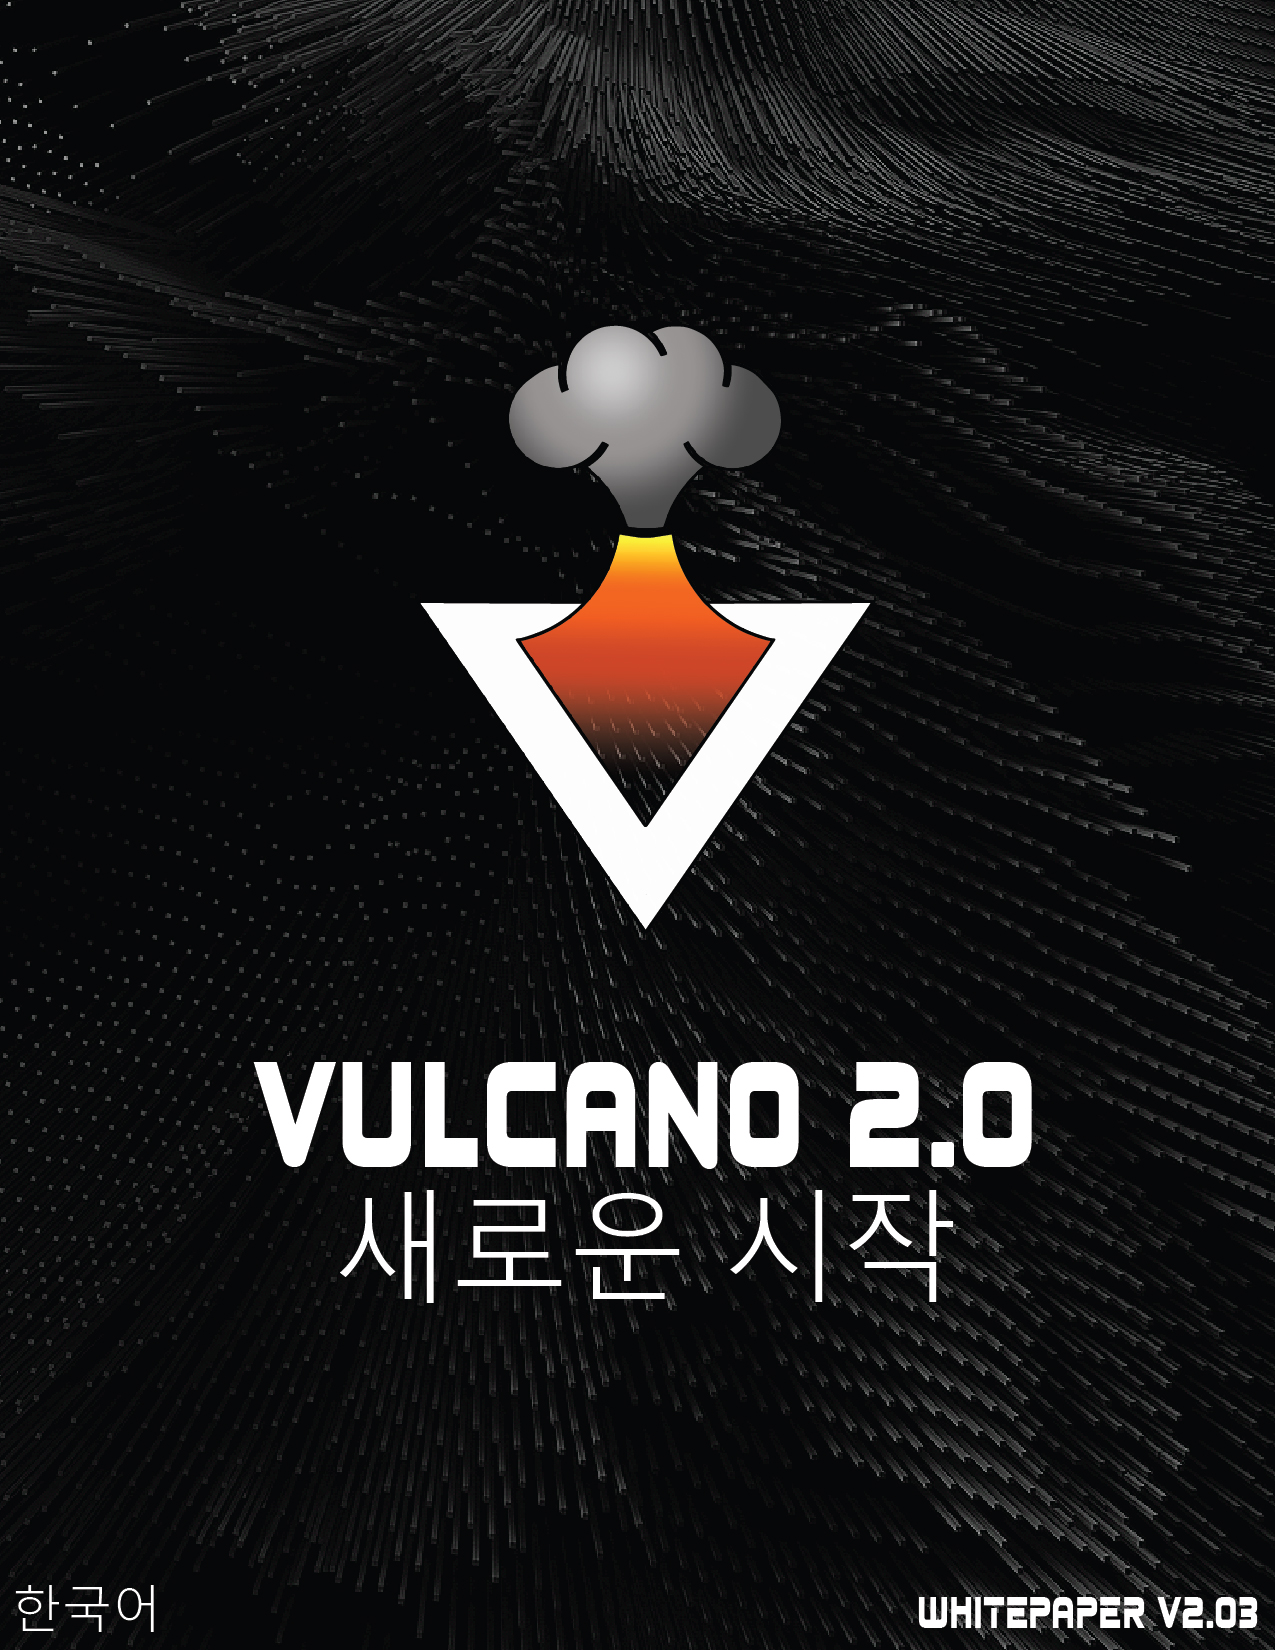
\includepdf[pages=1]{COVER-KOR.jpg}
\newpage
\tableofcontents
\newpage
\section{머릿말}

Vulcano(티커: VULC)는 현재는 사라진 개발팀이 원래 2017년말에 만든 커뮤니티 지향 코인입니다. 최초에는 연간 수익률이 950\%에 달하는 "고위험 코인"으로 인식됐지만, 최초 개발팀의 몇 가지 오류로 인해 실제 수익률은 320,000\%에 육박했습니다. 이 사실은 인식되지 않고 지나갔는데, 커뮤니티의 구성원 한 사람이 Genesis Block으로부터 블록체인을 검토함으로써 이 효과적인 수익률을 계산하게 됐습니다. . 이처럼 근본적인 약점이 노출되자, 커뮤니티의 구성원으로 이루어진 새로운 Vulcano 팀이 모여 기술적, 철학적 수준에서의 완전한 재구축과 실제 사용 사례의 개발을 통해 Vulcano 프로젝트를 살리고자 했습니다. 본 백서는 Vulcano의 완전한 업그레이드 전략과 업그레이드된 새로운 코인을 지열 탐사 자금에 투자하는 수단으로 다시 출범하는 내용을 다루고 있습니다.

당사는 단순히 Vulcano의 수익률 문제를 해결하는 데 그치지 않고, 새로운 코드 베이스로 코인을 완전히 업그레이드하기로 했습니다. Vulcano 팀은 Vulcano의 코어를 최고로 현대화하기 위해 Bulwark를 코드 베이스로 결정했습니다. Bulwark은 PIVX 위에 구축되었으며, PIVX는 그 자체가 널리 쓰이는 DASH 암호 화폐 위에 구축되어 있습니다. 이 중요한 결정으로 인해 당사는 매스터노드 기능인 거버넌스를 실행할 수 있을 것이고 궁극적으로 Vulcano 생태계를 지원하기 위한 하드웨어 노드를 통합할 수 있을 것입니다. 그 과정에서 당사는 거버넌스와 코인 스테이킹 및 네트워크 보안의 진정한 분산 시스템에 더욱 가까워질 것입니다.

본 백서에서는 또한 501(c)3 비영리 조직으로 구상하고 있는 Vulcano 재단의 설립을 통한 미국 내 Vulcano의 합법화도 다루고 있는데, 이를 통해 Vulcano는 자체적으로 성숙하게 성장하고 비즈니스 세계의 다른 부분과 연결하고 협상하게 될 것입니다. 이것이 특히 중요한 이유는 Vulcano의 장기 이용 사례에 아래에 설명할 연구 메커니즘을 통한 지적 자산 포트폴리오의 획득이 필요하기때문입니다. 전 세계 대학교 및 연구 기관에서의 연구에 자금 제공을 통해 지적 자산의 포트폴리오를 생성합니다. Vulcano 재단을 통해 이러한 지적 자산을 최고로 활용할 수 있을 것입니다. 이는 절대적으로 중요한 단계로서, 이를 통해 분산화된 Vulcano 프로젝트가 중앙집중화된 업계 및 학계와 상호작용하고 연결할 수 있습니다.

본 백서는 또한 미래의 개발을 위해 Vulcano 재단에 더 많은 자금을 조달할 수 있도록 과학을 발전시키고 지적 자산을 확보하면서 추가적인 보조금에 대한 자금을 조달할 수 있도록 하기 위한 지열 연구에 직접 자금을 대는 거버넌스 수수료의 계획 비율도 다룹니다.

이 백서에는 Vulcano 블록체인의 미래에 대한 터무니 없고 근거 없는 약속은 나오지 않습니다. Vulcano는 달성할 수 없는 약속을 하지 않고 혁신과 성장을 위해 노력하며, 대신 연구와 기술 개발의 진전에 노력을 기울일 것입니다. 본 백서에 언급된 모든 블록체인 기술은 이미 입증된 것이며 적절한 때에 활성화될 것입니다. 당사는 암호 화폐 커뮤니티가 자신들이 가져온 사업적 잠재력과 일관되게 행동을 시작해야 할 때가 되었으며, 기존 기술을 이용하는 데 대한 사업 타당성을 구축하기 위해 블록체인 기술에 대해 터무니 없는 주장을 할 필요가 없다고 믿습니다. 개발자, 팀의 리더들, 커뮤니티 자체가 더 폭넓은 업계 및 학계에 수용되기 위해서는 우리가 어느 정도 그들의 규칙에 따르려 해야 하고, 개발, 검증, 계획 이전에 입증되지 않은 블록체인 기술에 대한 아이디어를 펼치기 전에 이미 가진 것들을 효과적으로 이용해야 한다는 점을 이해해야 합니다. 미래에 Vulcano를 위한 블록체인 기술의 발전은 있겠지만, 그 출범은 수개월 간 팡파레와 마케팅에 수반되는 것이 아니고 개발된 이후에 말하게 될 것입니다. 당사는 이러한 "잠수함" 개발 방법이 화폐에 대한 최선의 방법이라고 믿습니다. 투기적 투자를 제한하고 미래 플랫폼의 안정적 기반을 구축할 수 있기 때문입니다.

Vulcano를 미래의 지속가능성에 대한 최고 자금원으로 변신시키고 궁극적으로 이 기술을 중심으로 사업 생태계를 구축하는 것이 당사의 목표입니다.

\section{감사의 말씀}
Bitcoin, Peercoin, Blackcoin, Talkcoin, Dash, PIVX, 또 특별히 Bulwark 팀의 이전 작업이 없었다면 Vulcano는 가능하지 않았을 것입니다. Vulcano의 새로운 탄생이 Bulwark의 한 갈래이므로, 본 백서의 일부 절은 그들의 백서에서 당사가 포함하지만 기존 코드 베이스에서 변형되지 않을 기능적인 부분을 그대로 차용했습니다. Vulcano 팀은 이러한 절을 다시 쓰면서 완전히 독창적인 척하는 것보다 Bulwark의 백서에 있는 그대로 포함시키는 것이 더욱 투명한 방법이라고 생각합니다.  커뮤니티로서 당사가 탄탄한 사용 사례와 광범한 세상을 위한 사업 구조를 개발하는 것이 중요하지만, 암호 화폐의 밑바탕인 오픈 소스 정신은 미래에도 계속 보호되고 유지되어야 합니다.  전반적으로 인류는 정보의 공유로 인한 혜택을 누릴 것이며, 당사는 이렇게 지식이 늘어나는 데 공헌함을 자랑스럽게 여깁니다. 당사가 Vulcano 재단을 통한 자금으로 개발된 기술을 Vulcano 생태계에 공헌한 나라들에 제공하는 것도 같은 정신에 따른 것입니다.

\section{암호 화폐에 대한 간단한 소개}
분산 원장 기술에 대한 제안은 1980년대 말로 거슬러 올라가지만, Satoshi Nakamoto라는 필명의 저자가 "Bitcoin: 피어 투 피어 전자 현금 시스템"이라는 제목의 논문을 무명의 암호 화폐 게시판에 발표하면서 진정한 블록체인이 탄생했습니다. 블록체인은 순서에 따라 거래에 타임스탬프를 찍고 이를 "블록"에 잠그며, 이를 훼손할 수 없도록 다양한 방법으로 인증함으로써 작동합니다. Bitcoin을 비롯한 많은 암호 화폐는 "작업 증명" 기반 위에서 운영되는데, 그 결과 계산 능력이 희소한 자원으로 작동하게 됩니다.

하지만 Vulcano는 지속가능성과 에너지 분야의 연구에 집중하기 때문에 이처럼 지속가능하지 않은 방법은 당사의 지속가능성 강화 노력과 상반됩니다. 그러므로, 당사는 "지분 증명" 기반으로 운영하기로 결정했으며, 여기에서는 네트워크의 희귀한 자원이 토큰 자체가 됩니다. 나아가, 본 백서의 게시 이후 30일 차에 발표될 업그레이드된 Vulcano의 출범과 함께 당사는지분 증명 방법의 다소 진보된 버전인 마스터노드를 갖게 될 것입니다. 여기에서는 세계의 컴퓨터들이 네트워크를 유지하지만 이 목적으로 간단한 계산을 일부 부담하게 됩니다. 지금 현재로서는 계산 부하가 간단한 스테이킹 지갑 운영보다 거의 크지 않지만, 당사는 이 네트워크를 미래에도 재생 에너지 업계의 화학 및 물리 계산 문제 운영을 위한 분산 컴퓨팅으로 쓸 것입니다.  이는 Vulcano의 장기 계획에 중요한 사항을 추가한 것입니다. 연구 대학교의 지질물리 및 지열 학과들은 대개 다른 매력적인 분야에 비해 자금 조달이 충분하지 않아서, 시뮬레이션을 수행하기 위한 대형 컴퓨터 사용 시간을 내기가 쉽지 않기 때문입니다.

나아가, 소비자 관점에서는, 90초의 블록 시간이 있는 매스터노드 합의 및 거래 잠금, 통제되고 안정화된 배출 일정, 친환경적 스테이킹 등 Vulcano는 진정으로 신속한 고기능 암호 화폐로 세계에 진정한 영향을 끼치지만 소비자와 암호 화폐 애호가에게 강력한 대안이 될 것입니다.

\section{새로운 Vulcano}
\subsection{새로운 Vulcano 블록체인의 세부 사항}

\begin{table}[h]
\centering
\begin{tabular}{@{}ll@{}}
\toprule
티커 & VULC \\ \midrule
알고리즘 & NIST5 \\
RPC 포트 & 62541 \\
P2P 포트 & 62543 \\
블록 스페이싱 & 90 초 \\
난이도 알고리즘 & Dark Gravity Wave v3.0 \\
블록 크기 & 1MB \\
채굴/생산 성숙도 & 67 블록 ($\sim$100 분) \\
확인 & 6 블록 ($\sim$9 분) \\
회람(1년) & 246,194,250 \\
회람(5년) & 421,126,225 \\
PoW 기간 & nHeight ≤ 60 \\
PoS 기간 & nHeight ≥ 61 \\
프로토콜 지원 & IPV4, IPV6, TOR \\
PoS & Blackcoin v3.0 PoS \\ \bottomrule
\end{tabular}
\end{table}

\subsection{커뮤니티를 함께 유지}
Vulcano는 원래 커뮤니티 코인으로 인식되었으며, 이는 당사가 전적으로 신뢰하는 개념입니다. 커뮤니티 코인으로서 당사는 프로젝트의 개발에 봉사하는 최선의 방법이 당사의 존재에 빚진 커뮤니티에 봉사하는 것임을 알고 있습니다. 당사는 현재의 레인, 콘테스트 등 커뮤니티 기반 활동을 계속할 것입니다. 또한 Vulcano 생태계의 한계에 대한 논의와 탐구도 촉진할 것입니다. 당사는 모든 포럼에서 신규 참여자, 사용자, 다른 암호 화폐 커뮤니티에 대한 괴롭힘에 대해 무관용 정책을 유지할 것입니다. Vulcano는 암호 화폐의 세상에 다른 프로젝트를 좌절시키기보다 함께 연결하고 시너지를 창출할 수 있으며 그래야만 하는 공간이 충분하다고 믿습니다. 다양한 암호 화폐 플랫폼의 지지자 간에 좋은 의미의 경쟁이 어느 정도 있을 수 있음을 이해하지만, 당사는 모든 상호 작용을 긍정적으로 유지하고자 합니다.

\subsection{사업 역량 구축}
이 백서를 쓰는 시점에 유사한 기술 기반을 활용하는 암호 화폐의 유입이 있었습니다. 기반이 되는 기술은 탄탄하지만, 세부 사양과 블록체인 매개 변수를 깊이 검토하면 공정하지 않은 관행이 드러나는 경우가 많습니다. 다른 경우에는, 기술적 실행이 열악하지만 커뮤니티가 문제에 대한 충분한 정보를 제공받지 않아 이를 판단할 수 없으며 근본적으로 건전하지 않은 프로젝트에 관여하기도 합니다.

애석하게도 원래의 Vulcano도 이러한 범주에 빠지기 쉬웠으며, 그 때문에 새로운 Vulcano 팀이 프로젝트를 전체적으로 수정하게 된 것입니다. 당사는 암호 화폐가 진정하게 사업적으로 적용이 되어야 하며, 이 기술이, 시장이 진정한 싩체를 이해하기 전에 움직이는 소수 보유자의 투기적 수입을 창출하는 데 쓰여서는 안 된다고 믿습니다. 개발자들이 나쁜 코인을 만들고, 매력적인 광고로 이를 밀어내고, 프로젝트를 포기함으로써 커뮤니티를 빈 수레로 만드는 일이 매우 잦습니다. 그래서 당사는 투명성과 책임성을 믿으며, 암호 및 비암호 세계 모두에서 진정한 사업을 하기 위해 필요한 사업적 기반을 확립할 것입니다. 

그러므로, 당사는 다수의 공식적 사업 조직을 만들어 이러한 상호 작용을 촉진하겠습니다. 처음이면서 가장 중요한 것은 지열 및 기타 지구 과학 연구 프로젝트에 자금을 지원할 목적으로 설립하는 501(c)3 비영리 조직입니다. 이 조직은 모든 지적 자산과 브랜딩 마크의 유지를 책임지게 됩니다.

또한 일련의 전 세계에 현지 요건에 따른 유한 회사를 설립할 것입니다. 많은 암호 화폐 거래소가 현지 사업체를 요구하며, LLC 네트워크를 구축함으로써 이를 충족할 수 있습니다. 이러한 네트워크틀 통해 Vulcano 재단과 Vulcano 커뮤니티는 세계 어디에서나 현지의 필요와 법적 요건을 준수하는 능력을 잃지 않고 사업을 수행할 수 있게 될 것입니다.

\subsection{커뮤니티 유지}
VULC 커뮤니티는 프로젝트의 장기적 성공에 가장 중요한 요인이며, 코인의 미래와 당사의 핵심 영역에서의 기술적 개발에 의미 있는 영향을 끼칠 수 있는 능력은  및 능력은 매우 중요합니다. 우리 발 밑에 있는 거의 무한한 지열의 힘을 통한 지속가능성에 대한 연구를 진행하는 것이 당사의 주요 목적이므로, 이 영역에 종사하는 연구자들에게 자금을 제공할 계획을 수립하였습니다.

그러므로, 당사의 첫해 말인 블록 172801에 당사는 네트워크 상에 예산 분출 블록을 활성화하려고 합니다. 이러한 분출 블록은 매월 지급되며 커뮤니티가 Vulcano가 자금을 대는 연구, 브랜드 존재의 개발, 커뮤니티 관련 행사를 의미 있게 통제할 수 있게 할 것입니다. 출범 이후 약 6개월 가량 이 시스템의 활성화를 늦춤으로써 당사는 긍정적인 사용자 경험에 필요한 기반 프레임워크를 개발할 시간을 얻게 되고, 시스템이 320,000\%에서 보다 합리적인 수치로 토큰 배출율을 낮추는 변화에서 안정화할 수 있습니다.

나아가, 10\%의 거버넌스 구조가 모든 블록 보상에 추가되며, 이는 지열 연구에 대해 투명하고 추적 가능하게 사용될 것입니다. 이것이 계속되면서, 당사는 당사 자체의 노력으로 선발하는 이외에 제안서 작성 및 제출의 다단계 절차를 활용할 것입니다. 제안서가 수락되려면, 선발 절차의 각 단계가 완전하게 충족되어야 합니다. 당사는 지혜와 지식이 다양한 곳에서 비롯된다고 믿기 때문에, Vulcano 커뮤니티가 지열 에너지 관련 기술에 대해 아이디어를 낼 것을 권장합니다.  이러한 제안과 아이디어들은 한데 가져와 다른 커뮤니티 사람들의 투표와 토론을 거친 후 학문적 수준에서 깊이 있게 탐구될 것입니다. Vulcano 커뮤니티가 전 세계의 지열 전문가에게 매력적이어서 이러한 아이디어 개발 과정에 참여할 수 있게 되는 것이 당사의 희망입니다.

\subsection{Vulcano 배출율}
아래는 Vulcano 블록체인의 블록 보상 및 배출율입니다.
\begin{table}[h]
\centering
\begin{tabular}{@{}ccccc@{}}
\toprule
월 & 블록 번호 & 블록 보상 & 배출 & 계 \\ \midrule
0 & 0-1 & 95,000,000 & 95,000,000 & 95,000,000 \\
1-6 & 2 to 172800 & 500 & 86,396,500 & 181,396,500 \\
7-12 & 172801 to 345600 & 375 & 64,797,750 & 246,194,250 \\
13-18 & 345601 to 518400 & 281.25 & 48,598,313 & 294,792,563 \\
19-24 & 518401 to 691200 & 210.94 & 36,448,734 & 331,241,297 \\
25-30 & 691201 to 864000 & 158.20 & 27,336,551 & 358,577,848 \\
31-36 & 864001 to 1036800 & 118.65 & 20,502,413 & 379,080,261 \\
37-42 & 1036801 to 1209600 & 88.99 & 15,376,810 & 394,457,071 \\
43-48 & 1209601 to 1382400 & 66.74 & 11,532,607 & 405,989,678 \\
49-54 & 1382401 to 1555200 & 50.06 & 8,649,456 & 414,639,133 \\
55-60 & 1555201 to 1728000 & 37.54 & 6,487,092 & 421,126,225 \\
61+ & 1728001 to Infinity & 18.77 & 계속 & 계속 \\ \bottomrule
\end{tabular}
\end{table}

\subsection{중앙집중을 이기기 위한 노력}
현존 블록체인 생태계에는 고질적인 문제가 다수 있습니다. 이러한 문제는 다양한 영역에 존재하기는 하지만 특정한 방식으로의 과도한 중앙집중화로 설명할 수 있습니다.

제거해야 할 첫 번째 중앙집중화 유형은 현존하는 토큰 혹은 코인의 절대 다수가 투기자들 손에 있다는 것입니다. 이는 다양한 주체들이 시장을 조작하고 정보를 갖고 있지 않은 투기자들이 다음 "대박"을 노리면서 급격하게 포지션을 사고 팔기 때문에 가격의 비합리적 등락으로 이어집니다. 이는 실제적 개발에 영향력이 적거나 없지만, 커뮤니티 내에 일부 방식의 가격 등락이 프로젝트의 기본적인 건강 상태를 결정하거나 반영한다는 태도를 만들게 됩니다. 둘 사이에는 아무 관계도 없는데도 그렇습니다. 투기자의 손에 있는 이러한 중앙집중화 문제는 변동성과 높은 위험으로 연결됩니다. 이러한 현상을 가능한 한 최대로 관리하는 것이 당사의 목표 중 하나입니다.

두 번째의 중앙집중화 유형은 마스터노드가 전형적으로 구성되는 가상 개인 서버 측면에서의 지역적 집중화입니다. 마스터노드의 호스팅을 싸게 제공하는 서비스로 인해 커뮤니티는 단일 서비스 제공자에 많은 수의 노드를 설치하는 경향이 있으며, 이는 예측하지 못한 한 가지 현상으로 인해 네트워크의 큰 부분이 지워질 수 있는 취약성을 의미합니다.

이러한 과도한 중앙집중화의 쌍둥이 문제의 해결책 중 하나는 Vulcano 연구 생태계입니다. Vulcano 재단이 지열 영역의 연구에 자금을 대므로, 지적 자산의 포트폴리오를 획득할 것이 기대됩니다. 당사의 계획은 이러한 지적 자산을 Vulcano 하드웨어 노드를 호스팅하는 데 동의한 모든 기관과 국가에 매우 낮은 비용으로 공급하는 것입니다.  이렇게 함으로써, 이 기관들은 자신들의 자체 시스템 혹은 Vulcano 하드웨어 노드에 마스터노드를 설치하는 단순한 비용으로 상당한 기술적 도구를 자신들의 기술에 대한 구성 요소로 이용할 수 있게 됩니다. 이렇게 함으로써 Vulcano 마스터노드는 지역적으로 더 크게 분산될 것이며, 커뮤니티에서 표류하며 투기에 이용될 토큰의 수는 줄어들 것입니다.

당사는 또한 Vulcano 토큰이 최대한 넓게 분산되는 것이 중요하다고 생각합니다. 사실상, 당사는 높은 비율의 토큰을 소수의 보유자 손에 준 소규모 암호 화폐 프로젝트의 다수가 프로젝트에 위험한 수준으로 중앙집중화되었다고 믿습니다. 그러므로, 당사는 미래에 분산화 및 대형 지갑의 분편화에 유인을 제공하고 적은 수의 마스터노드를 보유한 사람들에게 보상을 할 계획을 도입하려고 합니다. 이는 추후에 논의될 것입니다.
Vulcano 팀은 오픈 소스 개발의 강력한 옹호자이므로, 당사는 이처럼 오픈 소스에 가까운 사업 모드를 최대한 많은 영역에서 유지하고자 합니다. 물론, 모든 소스 코드는 항상 검사할 수 있을 뿐 아니라, 지적 자산의 실체를 최대한 비싸지 않게 이용할 수 있도록 제공할 것입니다.




\section{Vulcano의 특징}
\subsection {마스터노드}
전체적으로 마스터노드는 Vulcano 네트워크에 봉사하는 컴퓨터의 분산화된 웹입니다. 이들은 중요한 네트워크 기능을 수행하며 블록 보상의 일부를 받게 됩니다. 이러한 기본적 네트워크 기능에 봉사하는 이외에 코인 공급의 안정화, 거래 처리, 네트워크 보안을 통해 기여합니다. 마스터노드를 운영하려면 50,000 VULC와 적정한 기술적 지식이 필요합니다. 50,000 VULC 이상을 관리하는 지갑이라면 마스터노드를 설정할 수 있습니다.

Vulcano 팀은 유용한 계산 네트워크에 공헌하는 정도에 따라 보상을 받는 다양한 유형의 노드를 도입할 계획입니다. 이렇게 함으로써 수행되는 계산이 임의의 계산이 아니라 지속가능성과 연관된 과학의 진보에 공헌하는 기능적 계산이 되어 "작업 증명"의 어려움을 벗어날 수 있습니다. 추가적인 진전이 이뤄지면 추가적인 정보가 본 제안을 통해 발표될 것입니다.

\subsection{불명료화 / 코인 믹싱}
새로운 Vulcano의 핵심 코드가 Bulwark에 기초하고 있으므로, 이는 마스터노드의 네트워크에 의해 촉진되는 분산화된 방식으로 불명료화의 특징을 갖습니다. 이는 거래에 있어 프라이버시의 추가적인 레이어를 제공합니다. 완전한 익명은 아니지만, 노드 믹싱을 통한 불명료화는 표준적인 Bitcoin 거래보다 매우 우수합니다. 예를 들어, 모든 Bitcoin 거래는 투명하고 블록체인 전체에서 쉽게 추적할 수 있습니다. Vulcano에서는, 범죄 행위가가 운영 중인 마스터노드의 50\% 이상을 장악해야만 8라운드의 불명료화를 통해 혼합된 단일 거래의 익명성을 제거할 기회가 0.5\% 이상 될 것입니다. 이 중요한 기능은 자신의 거래를 불명료화하기로 선택한 VULC 사용자에게 높은 수준의 익명성을 제공하게 됩니다. 이는 Vulcano 프로젝트의 최종 사용 사례에 직접 연결되지는 않지만, 암호 화폐 단계에 있는 다른 프로젝트에 비해 가치를 확대할 수 있는 소비자 유용성 수준을 제공할 것입니다.

\subsection{SwiftTX}
SwiftTX는 마스터노드에 거래의 잠금 및 합의 권한을 부여합니다. 거래가 네트워크에 제출되면, 일단의 마스터노드가 거래 유효성을 확인할 것입니다. 이 마스터노드들이 거래 유효성에 대해 합의하게 되면 이는 잠겨져 추후 블록체인에 도입되며, 이를 통해 기존 시스템(Bitcoin의 경우 다수 확인을 위한 블록 시간이 10분)에 비해 거래 속도가 크게 향상됩니다. SwiftTX로 동일한 투입으로 네트워크의 한 블록을 채굴하기 전에 다수의 거래가 발생할 수 있습니다. 이 시스템은 Dash’s InstantSend에 기초하고 있습니다.

\subsection{스포크}
새로운 Vulcano 네트워크는 Bulwark가 도입한 다단계의 포크 메커니즘을 적용하며 이는 "스포킹"이라고 합니다. VULC 네트워크는 이를 이용해 새로운 기능을 실행하면서 출시 중 의도하지 않은 네트워크 포크의 가능성을 최소화할 수 있습니다. 스포크의 변경은 네트워크를 통해 배포되며 노드 소프트웨어의 업데이트 없이 필요에 따라 켜고 끌 수 있습니다. 이 기능은 매우 유용하며 이를 통해 개별 사용자가 수작업으로 지갑 코드를 변경하는 투입 없이 네트워크가 보안의 취약성에 신속하게 대응할 수 있습니다.

\subsection{TOR 및 IPV6 마스터노드}
Vulcano는 사용자들이 자신의 풀 노드 혹은 마스터노드를 어니언 주소 혹은 IPV6 주소에서 실행할 수 있게 할 것입니다. 당사는 풀 TOR 노드를 추가하여 TOR 네트워크 자체도 강화하고 TOR 전용 모드에서의 Bulwark 사용자 경험도 강화하고자 노력했습니다. TOR 마스터노드 지원의 독특한 특징은 마스터노드를 TOR 히든 서비스로 운영할 수 있다는 것입니다. TOR 노드를 이용하면 안정적 인터넷 연결을 가진 사용자들은 자신의 위치를 노출하는 프라이버시의 문제나 자신의 가정 네트워크를 공격이나 침해 가능성에 노출할 위험 없이 자신의 가정 네트워크에서 마스터노드를 운영할 수 있습니다.
 
\section{미래}
\subsection{Vulcano 안전 하드웨어 노드}
Vulcano 팀의 핵심 인력이 현재 소비자용 고급 전자제품 제조 전문업체와 함께 네트워크의 분산화와 상당한 수준의 보안을 제공할 수 있는 안전한 하드웨어 노드를 개발하고 있습니다. 사용자들은 자신의 가정 네트워크에서 여기에 접속하고 웹 UI를 이용해 구성할 수 있게 될 것입니다. 이는 안정적인 인터넷 연결을 가진 사람들을 위해 TOR 히든 서비스로 설치하기 쉬운, 완전 이온화된 마스터노드(혹은 풀 노드)와 함께 당사가 시작하려고 의도하는 기능입니다.

분산화의 정신을 유지하기 위해 모든 소스 코드는 커뮤니티에 제공되어 가정 어셈블리 뿐 아니라 기존 모델에도 제공될 것입니다. 이러한 노드들은 또한 Vulcano 재단이 정적 노드를 활용하여 지역적 분산화를 늘리고 코인 잠금을 향상하는 노력의 일환으로 배포할 노드입니다.

\subsection{Vulcano 매장}
당장 관심사가 되는 것은 Vulcano의 실세계 사용 사례를 만드는 것입니다. 그 첫 사례는 디지털 재화에 대한 시장으로 Vulcano 블록체인에서 운영됩니다. 처음에는 Steam 코드와 상품권처럼 커뮤니티 외부에서 오는 디지털 재화에 대한 것이 되겠지만 Vulcano에 기초한 피어 투 피어 마켓플레이스로 확장될 계획입니다.

\subsection{텔레그램 및 디스코드 보트}
모든 블록체인 프로젝트의 핵심은 커뮤니티이며, 커뮤니티에 봉사하는 가장 큰 방법 중 하나는 커뮤니티에 의사 소통하고 토큰을 이용할 방법을 제공하는 것입니다. Vulcano 팀은 다양한 채팅 서비스를 위한 보트를 개발할 것이며, 이를 이용하면 사람들은 자신의 VULC를 세계와 쉽게 공유할 수 있습니다. Vulcano를 이렇게 자유롭게 흐르게 함으로써 당사는 커뮤니티에 참여하고 커뮤니티를 성장시키면서 효용을 확대할 수 있습니다.

\section{결론}
Vulcano는 수 개월 전 심각한 약점이 처음 발견된 상태에서 멀리 왔습니다. 새로운 Vulcano 체인에 대한 검증이 진행되고, 기능이 확대되고, 수개월 동안 프로젝트와 커뮤니티에 장애가 되었던 문제를 해결하기 위한 노력이 많이 진행됐습니다. 당사는 이러한 변화 및 업그레이드를 발표할 수 있게 되고, 당사의 장기적 계획을 알리게 되어 기쁘게 생각합니다. 본 백서는 살아 있는 문서로 지속적인 업데이트를 제공하게 되기를 기대합니다.
\newpage
\section{Changelog}

\begin{table}[h]
\centering
\begin{tabular}{@{}ccccc@{}}
\toprule
번역 & 당일 & 설명 \\ \midrule
v2.03 KR & August 8th, 2018 & 첫 번째 번역 \\
 \bottomrule
\end{tabular}
\end{table}

\end{document}
